%%%%%%%%%%%%%%%%%%%%%%%%%%%%%%%%%%%%%%%%%%%%%%%%%%%%%%%%%%%%%
% Programmer : Joseph Vitale
% Date : 02/15/21
% Assessment : CDR Puzzle Me Chess
%%%%%%%%%%%%%%%%%%%%%%%%%%%%%%%%%%%%%%%%%%%%%%%%%%%%%%%%%%%%%

\documentclass[11pt]{article}

%%%%%%%%%%%%%%%%%%%%%%%%%%%%%%%%%%%%%%%%%%%%%%%%%%%%%%%%%%%%%
% Change "article" to "report" to get rid of page number on title page
% Most of these packages that you are calling will be installed by MiKTeX the first time you use it
% After that, they should work fine on your jump drive or laptop
%%%%%%%%%%%%%%%%%%%%%%%%%%%%%%%%%%%%%%%%%%%%%%%%%%%%%%%%%%%%%

\usepackage{amsmath,amsfonts,amsthm,amssymb}
\usepackage{setspace}
\usepackage{Tabbing}
\usepackage{fancyhdr}
\usepackage{lastpage}
\usepackage{extramarks}
\usepackage{chngpage}
\usepackage{soul,color}
\usepackage{graphicx,float,wrapfig}
\usepackage{graphicx}
\graphicspath{ {images/} }

%%%%%%%%%%%%%%%%%%%%%%%%%%%%%%%%%%%%%%%%%%%%%%%%%%%%%%%%%%%%%
% In case you need to adjust margins:
\topmargin=-0.45in      %
\evensidemargin=0in     %
\oddsidemargin=0in      %
\textwidth=6.5in        %
\textheight=9.0in       %
\headsep=0.25in         %
%
%%%%%%%%%%%%%%%%%%%%%%%%%%%%%%%%%%%%%%%%%%%%%%%%%%%%%%%%%%%%%
%%%%%%%%%%%%%%%%%%%%%%%%%%%%%%%%%%%%%%%%%%%%%%%%%%%%%%%%%%%%%
% Homework Specific Information (THIS IS WHERE YOU MAKE YOUR TITLE CHANGES)
%
% You only need to change the homework number and the Date
%
% You should make sure your correct name is on this as well.
%
\newcommand{\hmwkTitle}{Puzzle Me Chess}
\newcommand{\hmwkDueDate}{February\ 22,\ 2021}
\newcommand{\hmwkClass}{Critical Design Review}
\newcommand{\hmwkClassInstructor}{EN.525.743.8VL.SP21}
\newcommand{\hmwkAuthorName}{Mr. Joseph Vitale}

%
%
%
%%%%%%%%%%%%%%%%%%%%%%%%%%%%%%%%%%%%%%%%%%%%%%%%%%%%%%%%%%%%%
%%%%%%%%%%%%%%%%%%%%%%%%%%%%%%%%%%%%%%%%%%%%%%%%%%%%%%%%%%%%%
% Set up for the header and footer here
% This stuff should not change much for you, but you may play around with it safely.
% Notice that the "\lhead" is for the left header and "\chead" is for the center header, etc.

\pagestyle{fancy}                                                      
\lhead{\hmwkAuthorName}                                                 
\chead{\hmwkClass\ (\hmwkClassInstructor )}  
\rhead{\firstxmark}                                                     
\lfoot{\lastxmark}                                                      
\cfoot{}                                                                
\rfoot{Page\ \thepage\ of\ \pageref{LastPage}}                          
\renewcommand\headrulewidth{0.4pt}                                      
\renewcommand\footrulewidth{0.4pt}   
                                   

%%%%%%%%%%%%%%%%%%%%%%%%%%%%%%%%%%%%%%%%%%%%%%%%%%%%%%%%%%%%%
% Tools to mark the numbering of problems. They don't need to be modified by you.
% All the text below is pretty important for the formatting, but you don't need to change it.
%
\newcommand{\enterProblemHeader}[1]{\nobreak\extramarks{#1}{#1 continued on next page\ldots}\nobreak%
                                    \nobreak\extramarks{#1 (continued)}{#1 continued on next page\ldots}\nobreak}%
\newcommand{\exitProblemHeader}[1]{\nobreak\extramarks{#1 (continued)}{#1 continued on next page\ldots}\nobreak%
                                   \nobreak\extramarks{#1}{}\nobreak}%

\newlength{\labelLength}
\newcommand{\labelAnswer}[2]
  {\settowidth{\labelLength}{#1}%
   \addtolength{\labelLength}{0.25in}%
   \changetext{}{-\labelLength}{}{}{}%
   \noindent\fbox{\begin{minipage}[c]{\columnwidth}#2\setlength{\parindent}{10mm}\end{minipage}}%
   \marginpar{\fbox{#1}}%

   % You can leave this alone too
   \changetext{}{+\labelLength}{}{}{}}%

% Nothing to change here
\setcounter{secnumdepth}{0}
\newcommand{\homeworkProblemName}{}%
\newcounter{homeworkProblemCounter}%
\newenvironment{homeworkProblem}[1][Problem \arabic{homeworkProblemCounter}]%
  {\stepcounter{homeworkProblemCounter}%
   \renewcommand{\homeworkProblemName}{#1}%
   \section{\homeworkProblemName}%
   \enterProblemHeader{\homeworkProblemName}}%
  {\exitProblemHeader{\homeworkProblemName}}%

\newcommand{\problemAnswer}[1]
  {\noindent\fbox{\begin{minipage}[c]{\columnwidth}#1\setlength{\parindent}{10mm}\end{minipage}}}%

\newcommand{\problemLAnswer}[1]
  {\labelAnswer{\homeworkProblemName}{#1}}

\newcommand{\homeworkSectionName}{}%
\newlength{\homeworkSectionLabelLength}{}%
\newenvironment{homeworkSection}[1]%
  {% The author put this space here to make sure it is not connected to the above.
   % Otherwise the changetext can do funny things to the other margin

   \renewcommand{\homeworkSectionName}{#1}%
   \settowidth{\homeworkSectionLabelLength}{\homeworkSectionName}%
   \addtolength{\homeworkSectionLabelLength}{0.25in}%
   \changetext{}{-\homeworkSectionLabelLength}{}{}{}%
   \subsection{\homeworkSectionName}%
   \enterProblemHeader{\homeworkProblemName\ [\homeworkSectionName]}}%
  {\enterProblemHeader{\homeworkProblemName}%

   % The author put the blank space above in order to make sure this margin
   % change doesn't happen too soon (otherwise \sectionAnswer's can
   % get ugly about their \marginpar placement.
   \changetext{}{+\homeworkSectionLabelLength}{}{}{}}%

\newcommand{\sectionAnswer}[1]
  {% The author put this space here to make sure we're disconnected from the previous
   % passage

   \noindent\fbox{\begin{minipage}[c]{\columnwidth}#1\setlength{\parindent}{10mm}\end{minipage}}%
   \enterProblemHeader{\homeworkProblemName}\exitProblemHeader{\homeworkProblemName}%
   \marginpar{\fbox{\homeworkSectionName}}%

   % The author put the blank space above in order to make sure this
   % \marginpar gets correctly placed.
   }%
%
% All the text above is pretty important for the formatting, but you don't need to change it.
%
%%%%%%%%%%%%%%%%%%%%%%%%%%%%%%%%%%%%%%%%%%%%%%%%%%%%%%%%%%%%%


%%%%%%%%%%%%%%%%%%%%%%%%%%%%%%%%%%%%%%%%%%%%%%%%%%%%%%%%%%%%%
%    Formatting the title. This part of the document is where the title page is set up.
%    We are almost to the beginning of the homework!
%
\title{\vspace{2in}\textmd{\textbf{\hmwkClass:\ \hmwkTitle}}\\\normalsize\vspace{0.1in}\small{\hmwkDueDate}\\\vspace{0.1in}\large{\textit{\hmwkClassInstructor\ }}\vspace{3in}}
\date{}
\author{\textbf{\hmwkAuthorName}}

%
%
%
%%%%%%%%%%%%%%%%%%%%%%%%%%%%%%%%%%%%%%%%%%%%%%%%%%%%%%%%%%%%%
%%%%%%%%%%%%%%%%%%%%%%%%%%%%%%%%%%%%%%%%%%%%%%%%%%%%%%%%%%%%%
%%%%%%%%%%%%%%%%%%%%%%%%%%%%%%%%%%%%%%%%%%%%%%%%%%%%%%%%%%%%%
%  This is the BEGINNING of the DOCUMENT
%
%
\begin{document}

\maketitle % Actually calling the typesetter to include the title that you formatted above
\newpage
% Comment out the \tableofcontents and \newpage lines to get remove the Contents page
% Uncomment the \setcounter line as well if you do NOT want subsections
%       listed in Contents
%\setcounter{tocdepth}{1}

\tableofcontents % 
%\newpage % The \\ command tells LaTeX to start a new line. 

% When problems are long, it may be desirable to put a \newpage or a
% \clearpage before each homeworkProblem environment

\clearpage 
% The \clearpage command ends the current page and causes all figures 
% and tables that have so far appeared in the input to be printed.
%%%%%%%%%%%%%%%%%%%%%%%%%%%%%%%%%%%%%%%%%%%%%%%%%%%%%%%%%%%%%%%%%%%%%%%%%%%%%%%%%%%%%%%%%%%%%%%%%%%%%%%%%%%%%%%%%%
\section{Project description}
In chess there are many different ways to play the game. After each player moves three times there are 121 million different moves that can end the game. Many people need to practice chess in order to get better and there are many ways to do this. You can play over the internet and play computer which range from (400 - 3200) EIO or you can play puzzle's in chess. Puzzle's in chess allow you to study the board in a given state and make the next several moves. This project is dedicated to solving puzzles in the physical world. 
\\

\noindent The physical chess puzzle allows the user to practice looking at a physical board to solve each puzzle. This project is titled "Puzzle me Chess`` and it will be equipped to have 3 different puzzle's. The chess board will allow the user to place each piece in the right location that is displayed on the OLED screen. After each piece is on the board the chess puzzle will then display to the user which color he/she will play. After the user makes his first move the board will check to see if the move was correct. If not the user will be asked to reset the piece and try again until puzzle is complete. 

\subsection{Capabilities}
Capabilites for the Puzzle me Chess project range from Indicators, User Direction, SD card capability, and Location Detection. See below for more details. 

\begin{center}
    \begin{tabular}{| l | l |}
    \hline
    Capability  & Description below\\ \hline
    Indicator &  LED light indicator to show user hint/show answer feature \\ \hline
    User Direction & OLED to describe to the user where to put pieces \\ \hline 
    SD Card & Read .csv standardized format to quickly import puzzles \\ \hline
    User Direction & User input switch to show user answer, indicated by LEDs \\ \hline
    User Direction & User input Button to show user a hint \\ \hline
    Location Detection & Check board spots are correct for puzzle that was selected \\ \hline
    \end{tabular}
\end{center}
 *Assume User puts right pieces on spot 
 \newline
 *Assume Chess Board will be lit evenly with light  
\subsection{Limitations}
Limitations for the Puzzle me Chess project range from Location Detection, Auto Movement, Puzzle Selection, Physical and parts. See below for more details.

\begin{center}
    \begin{tabular}{| l | l |}
    \hline
    Limitations  & Description below\\ \hline
    Location Detection & Not knowing which piece is on the spot \\ \hline
    Auto Movement & Not being able to move the piece on correct spot \\ \hline 
    Puzzle Selection & Not having 3+ different puzzles to choose from  \\ \hline
    Physical & Not being able to light each square along the perimeter  \\ \hline
    Parts & Not having multiple colors to indicate wrong or right answer \\ \hline
    Physical & Needing light to illuminate  the chess board \\ \hline
    \end{tabular}
\end{center}

\section{Functional description}
The Puzzle me Chess project will feature a microcontroller, one 21x21 wooden chess board, 8 Multiplexers, 1 switch, 1 Potentiometer, 1 button, and A Display. Figure \ref{fig:Circuit} shows  the current circuit layout as of 02/16/2021, this circuit doesn't show the chess board. Explanation of the System Block Diagram to follow.

\begin{figure}
  \includegraphics[width=\linewidth]{./Pics/Circuit_as_of_2162020.jpg}
  \caption{Circuit layout as of 02/16/2021}
  \label{fig:Circuit}
\end{figure}

\subsection{System Block Diagram}
Figure \ref{fig:SBD1} shows the sudo hand drawn block diagram. The project consist of One Microcontroller which will feature the teensy 3.6, 8 Multiplexer's from Texas Instruments part \# CD4051BE, 1 basic breadboard switch, 1 breadboard Potentiometer, 1 basic breadbaord button, LED's, Photoresister's, 1 Chess Board and one Display. 
\\


\noindent The Chess board will have 1 LED and 1 photoresister per block. The LED will be drilled and placed on the top left side of each block and will be used to show the user where to place each piece. The photoresister will be drilled in the middle of each block and will be used as a voltage drop to tell if there is a piece there or not. See section multiplexer circuit diagram for the circuit layout. 

\begin{figure}
  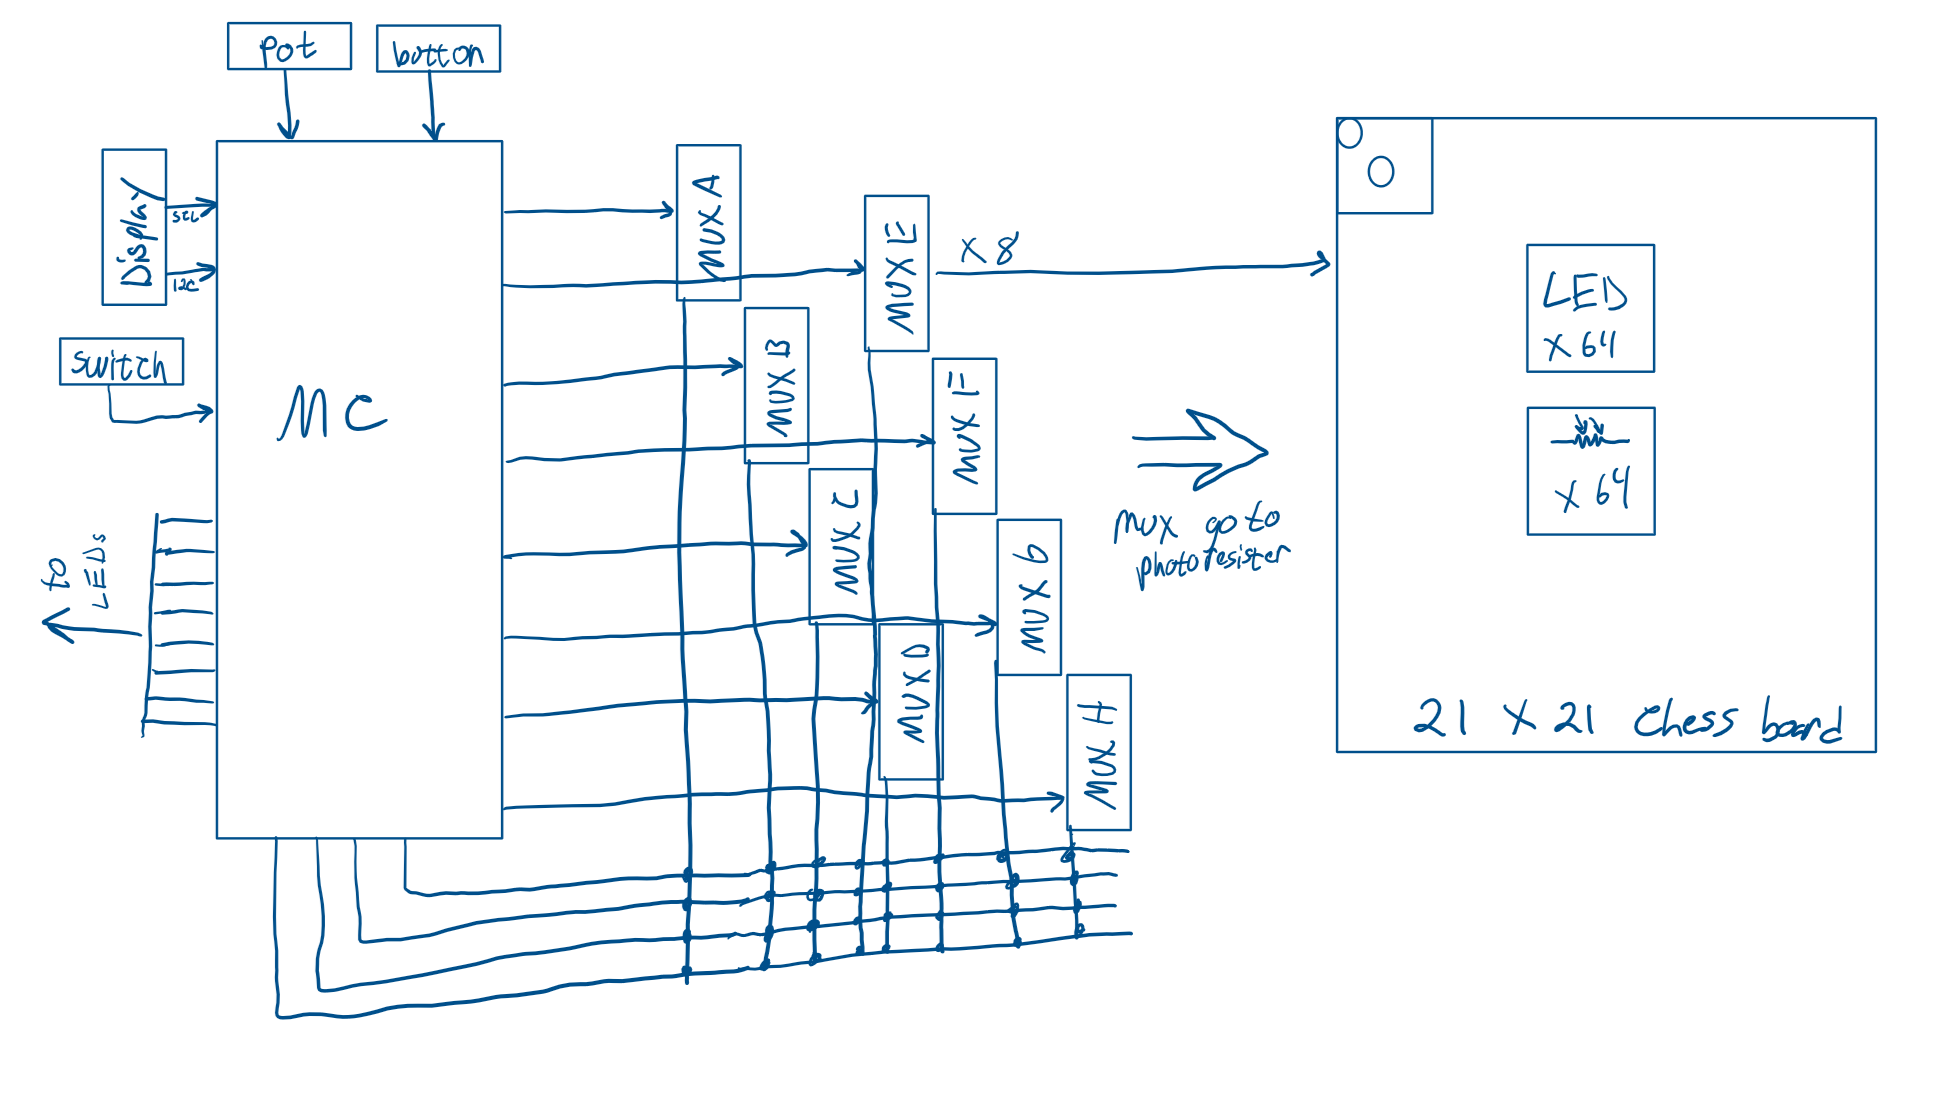
\includegraphics[width=\linewidth]{./Pics/System_Block_Diagram.PNG}
  \caption{System Block Diagram}
  \label{fig:SBD1}
\end{figure}

% Figure \ref{fig:boat1} shows a boat.

\subsection{Multiplexer Circuit Diagram} 
Figure \ref{fig:MSCD} shows the sudo circuit for Muxltiplexer A, the puzzle me chess project will consist of 8 Muxltiplexer one for each column A-H. Each of the Muxltiplexers will have 8 outgoing lines that will read Voltages levels from the column and rows \# 1-8. Each row will have one resister which will be $~2M \Omega$ and one Photoresister in series. Each Photoresister has two modes a light and a dark mode. Equation
\\


Assume Light; R = $500 \Omega$
\\


Assume Dark; R = $1M \Omega$


\begin{equation}
Light
$$ V = IR, 3.3VDC = I*(2M + 500)$\Omega$ $$
$$ I = 1.65$\mu$A, Vlight = 825$\mu$VDC, Mux input would see 3.299VDC if no piece on top of photoresister$$
\end{equation}

\begin{equation}
Dark
$$ V = IR, 3.3VDC = I*3.3M$\Omega$ $$
$$ I = 1.1$\mu$A, Vdark = 1.1VDC, Mux input would see 2.2VD  if piece was placed on block$$
\end{equation}
\begin{figure}
  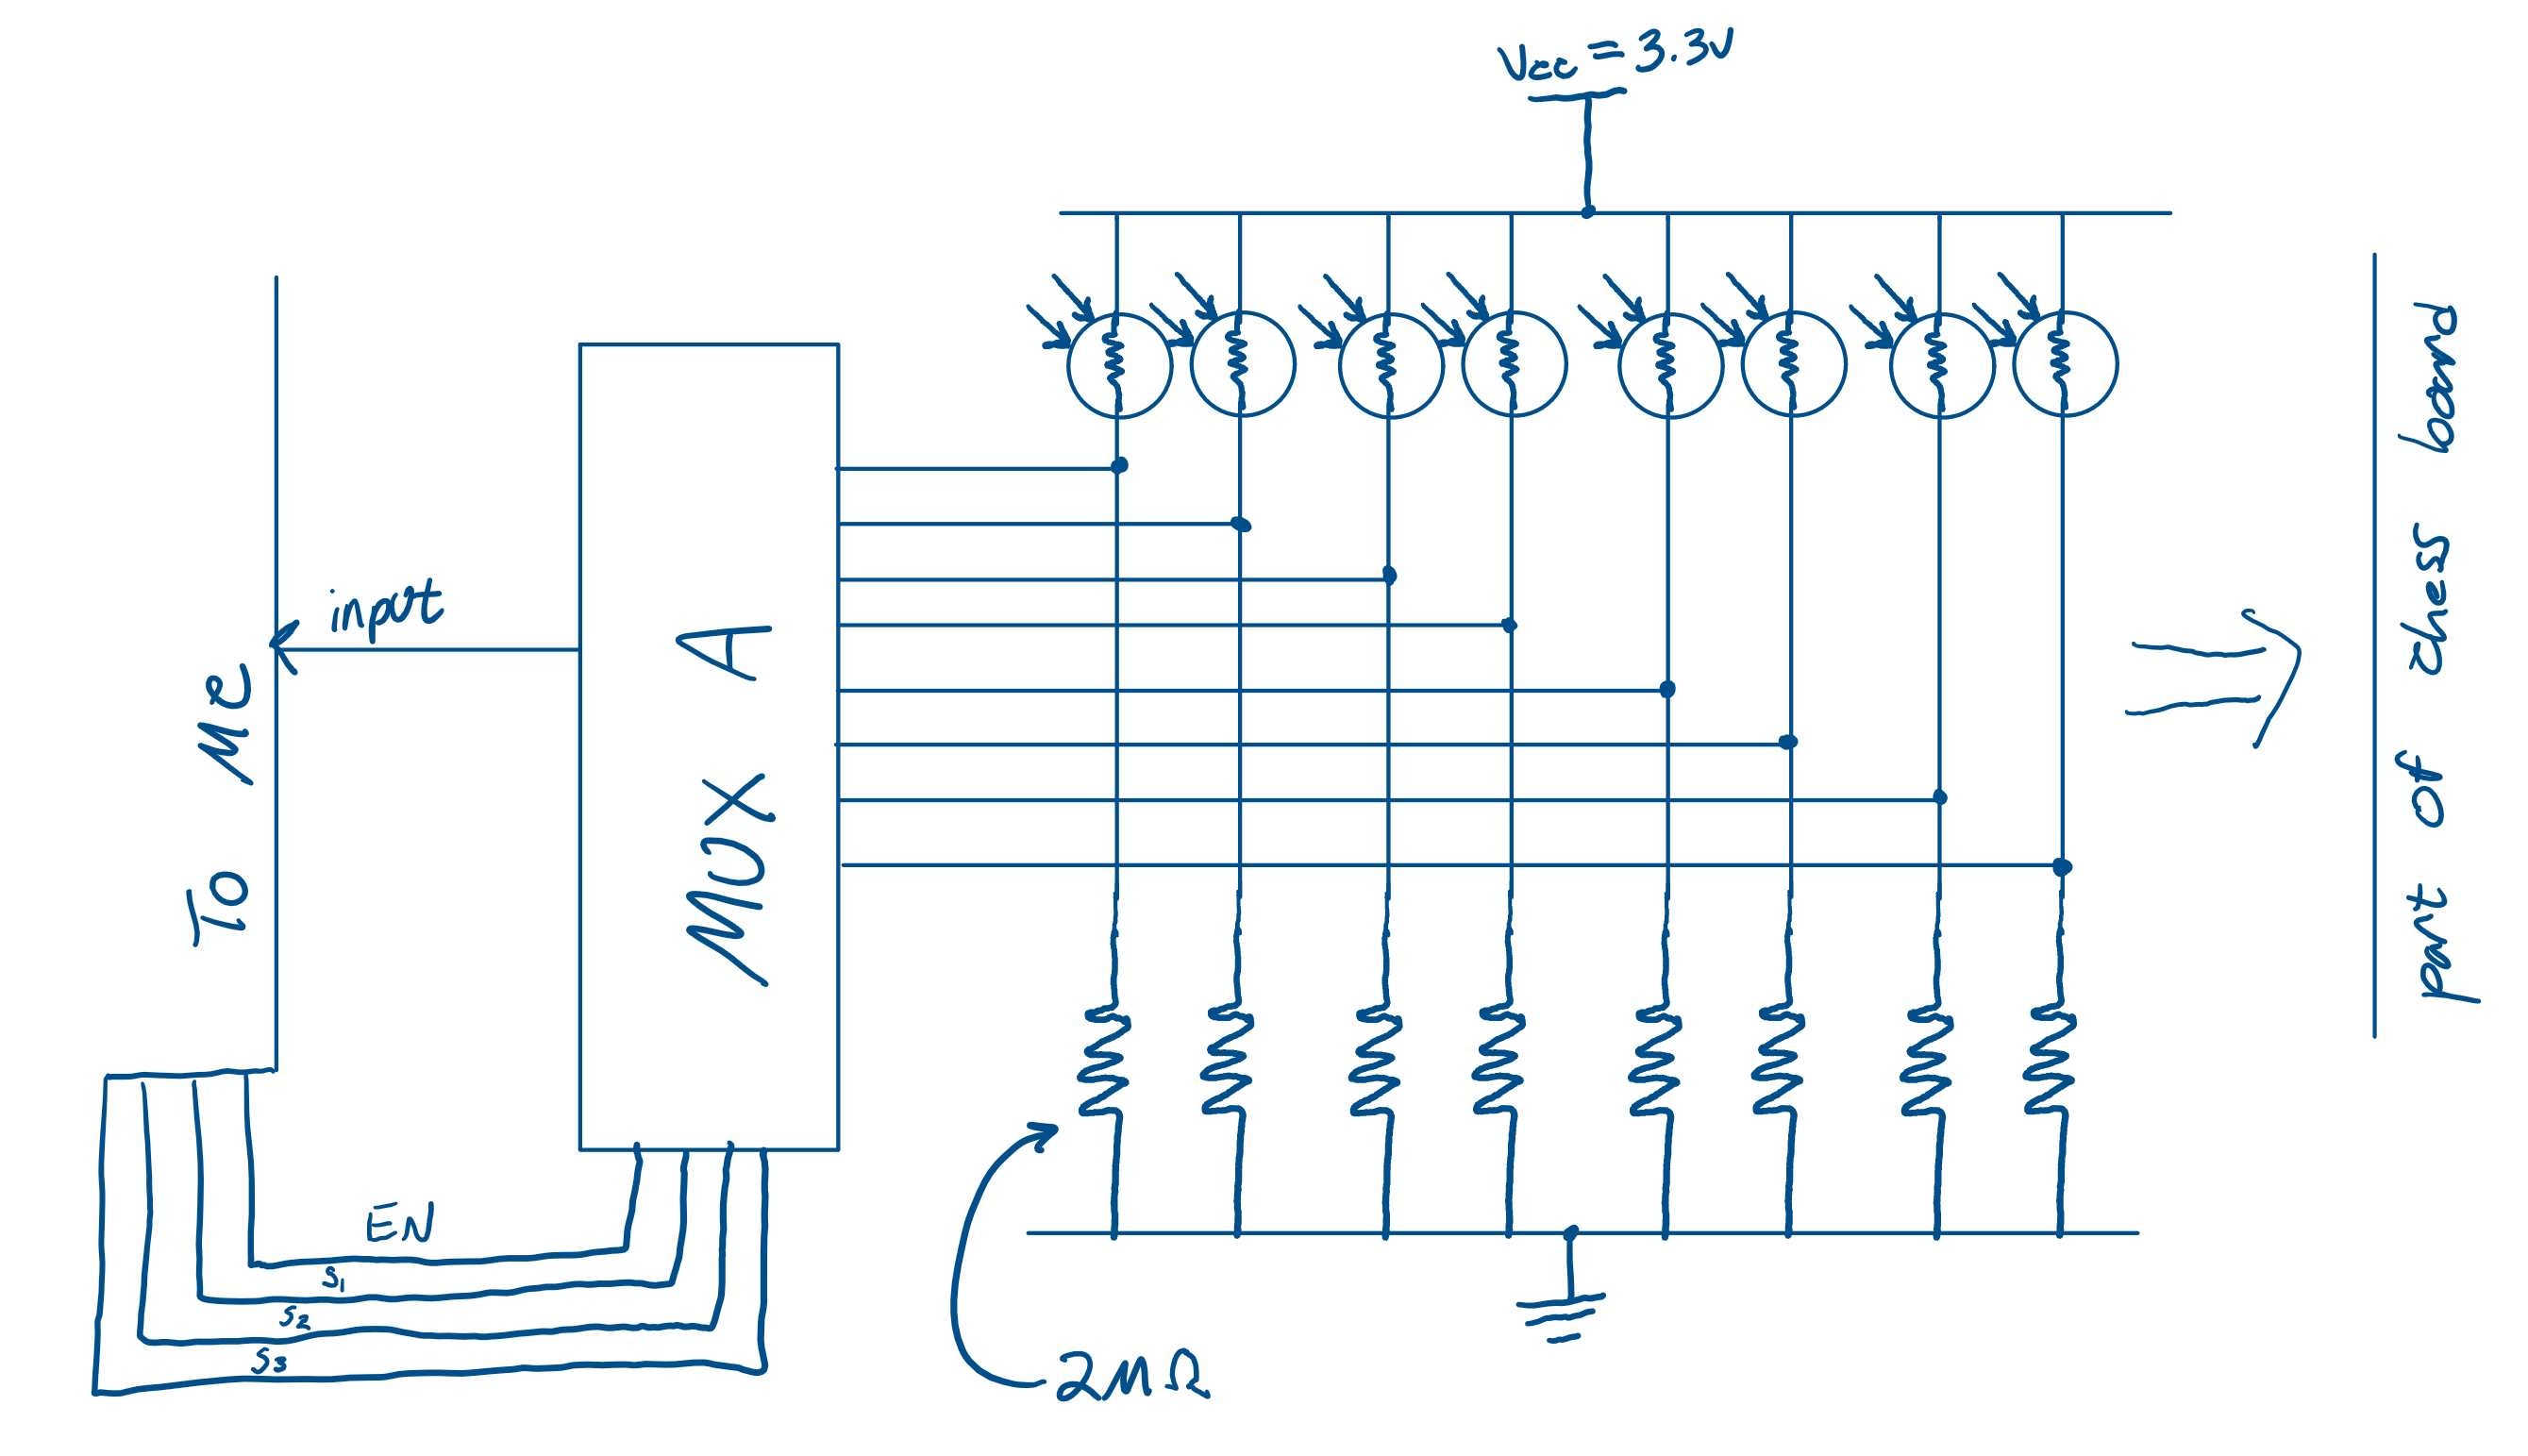
\includegraphics[width=\linewidth]{./Pics/Mux_sudo_circuit.PNG}
  \caption{Multiplexer Sudo Circuit Diagram}
  \label{fig:MSCD}
\end{figure}


\subsection{Code Flow Diagram}

\begin{center}
\begin{figure}
  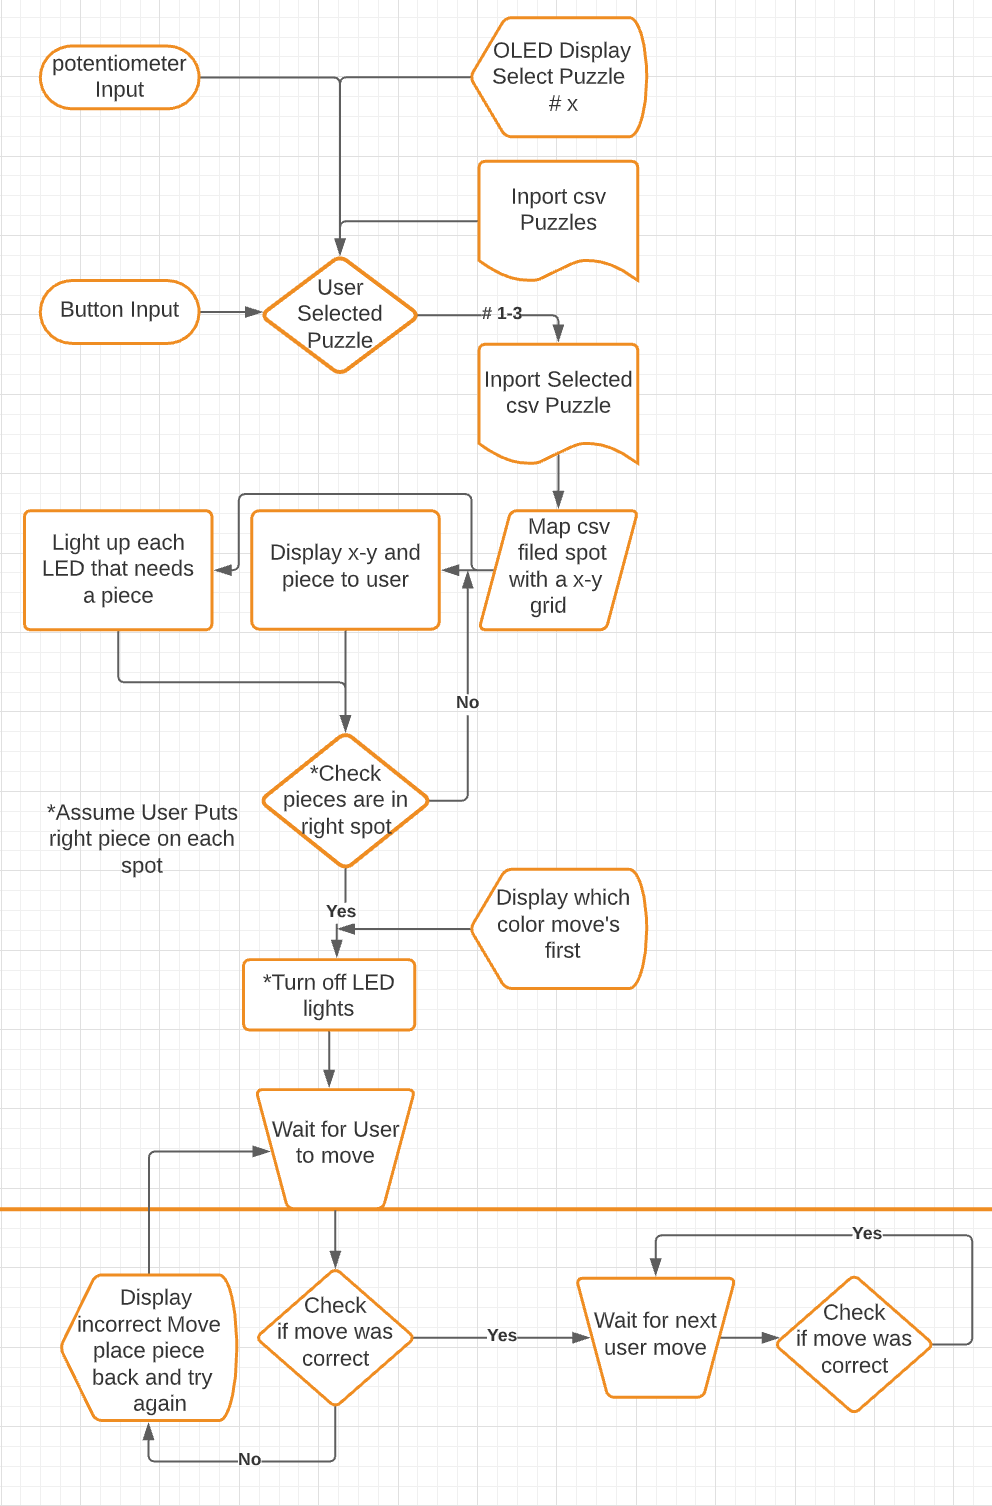
\includegraphics[width=17cm,height=21cm]{./Pics/Code_Flow_Diagram.PNG}
  \caption{Code Flow Diagram}
  \label{fig:CFD1}
\end{figure}
\end{center}

\section{Interface description}
\subsection{Internal}

\section{Explanation of code}
Text Text
\subsection{Code layout}

\begin{figure}
  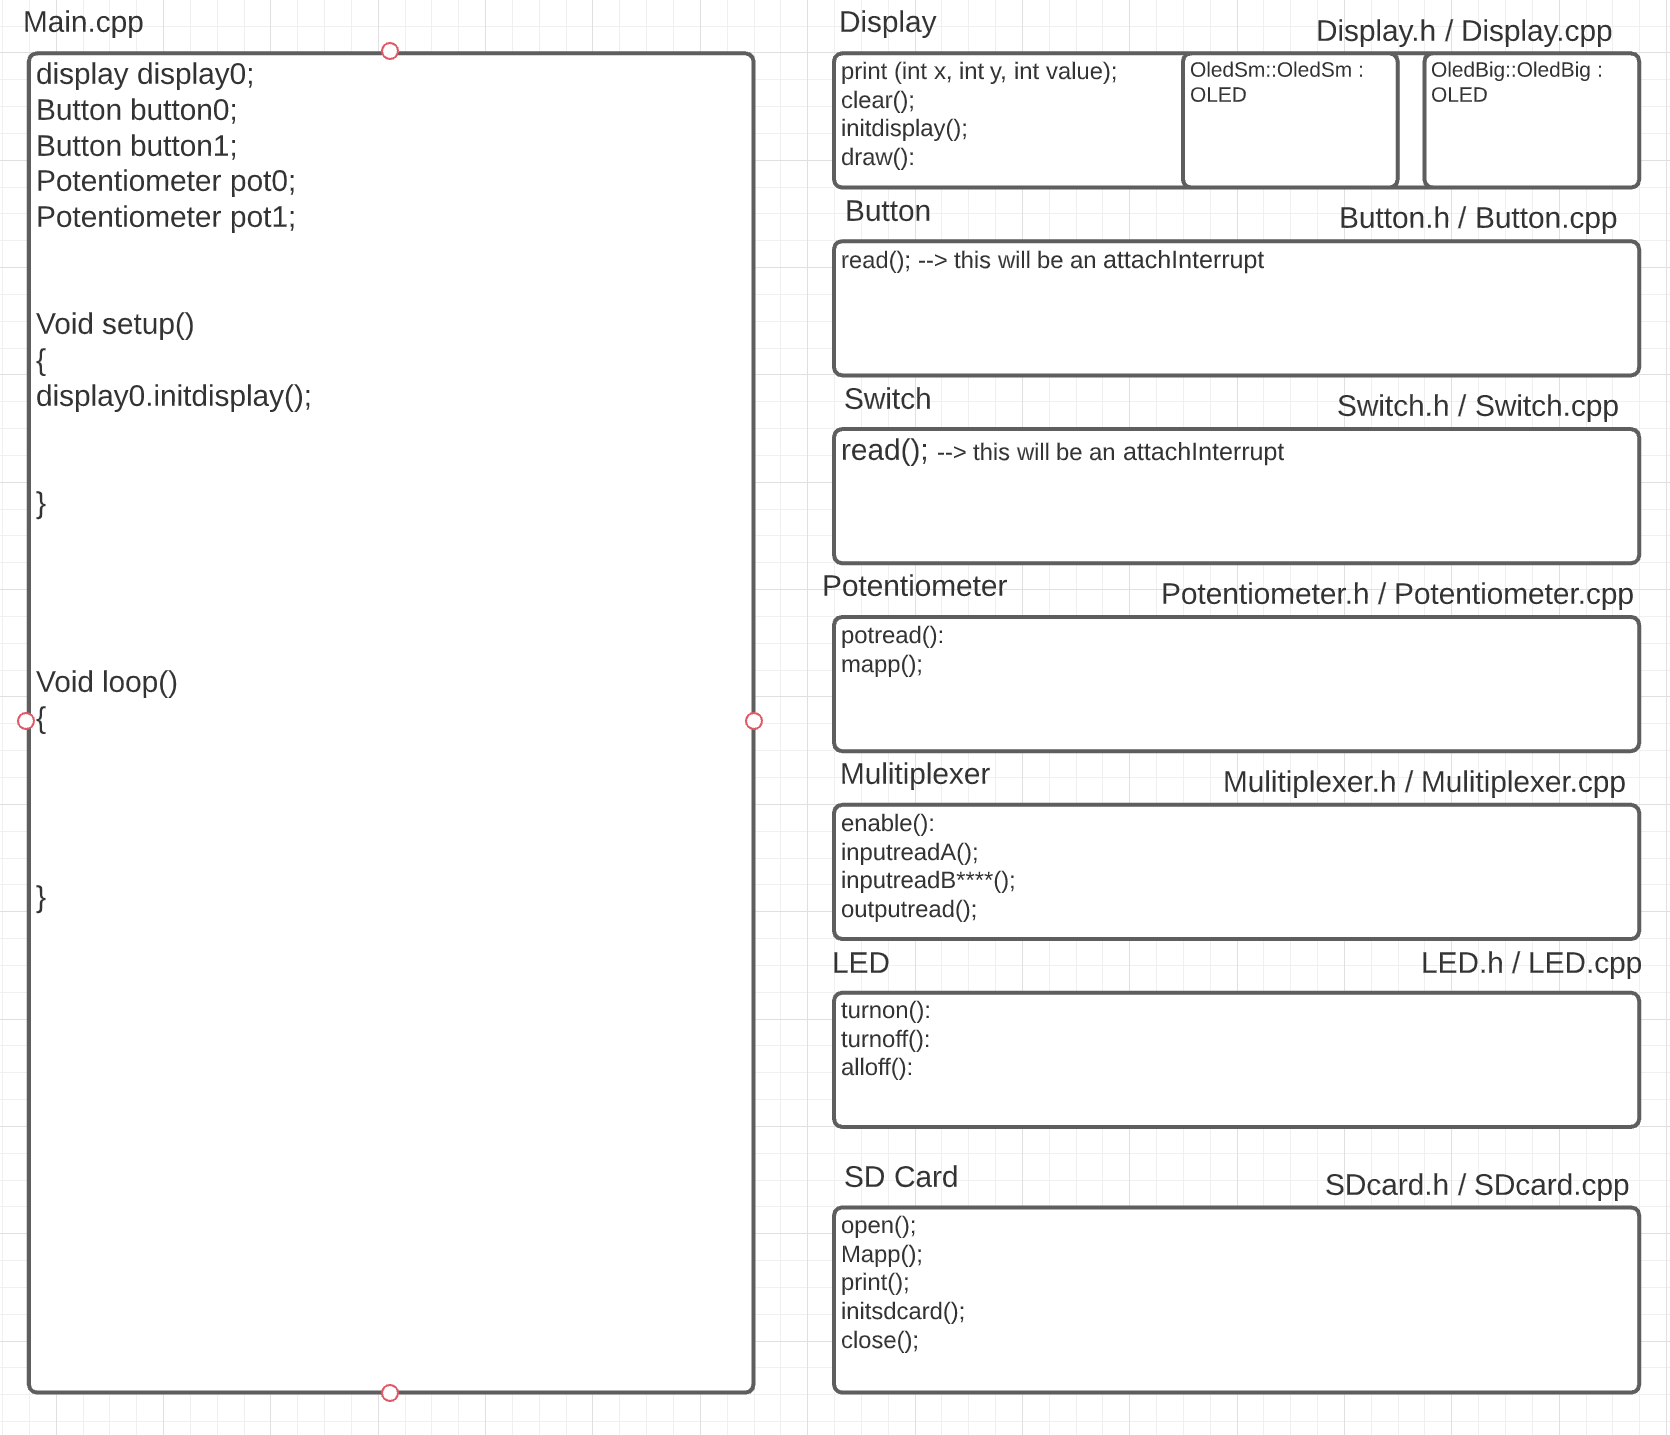
\includegraphics[width=\linewidth]{./Pics/code_layout.PNG}
  \caption{Module Code Layout}
  \label{fig:MCL1}
\end{figure}

\subsection{Main}

\begin{figure}
  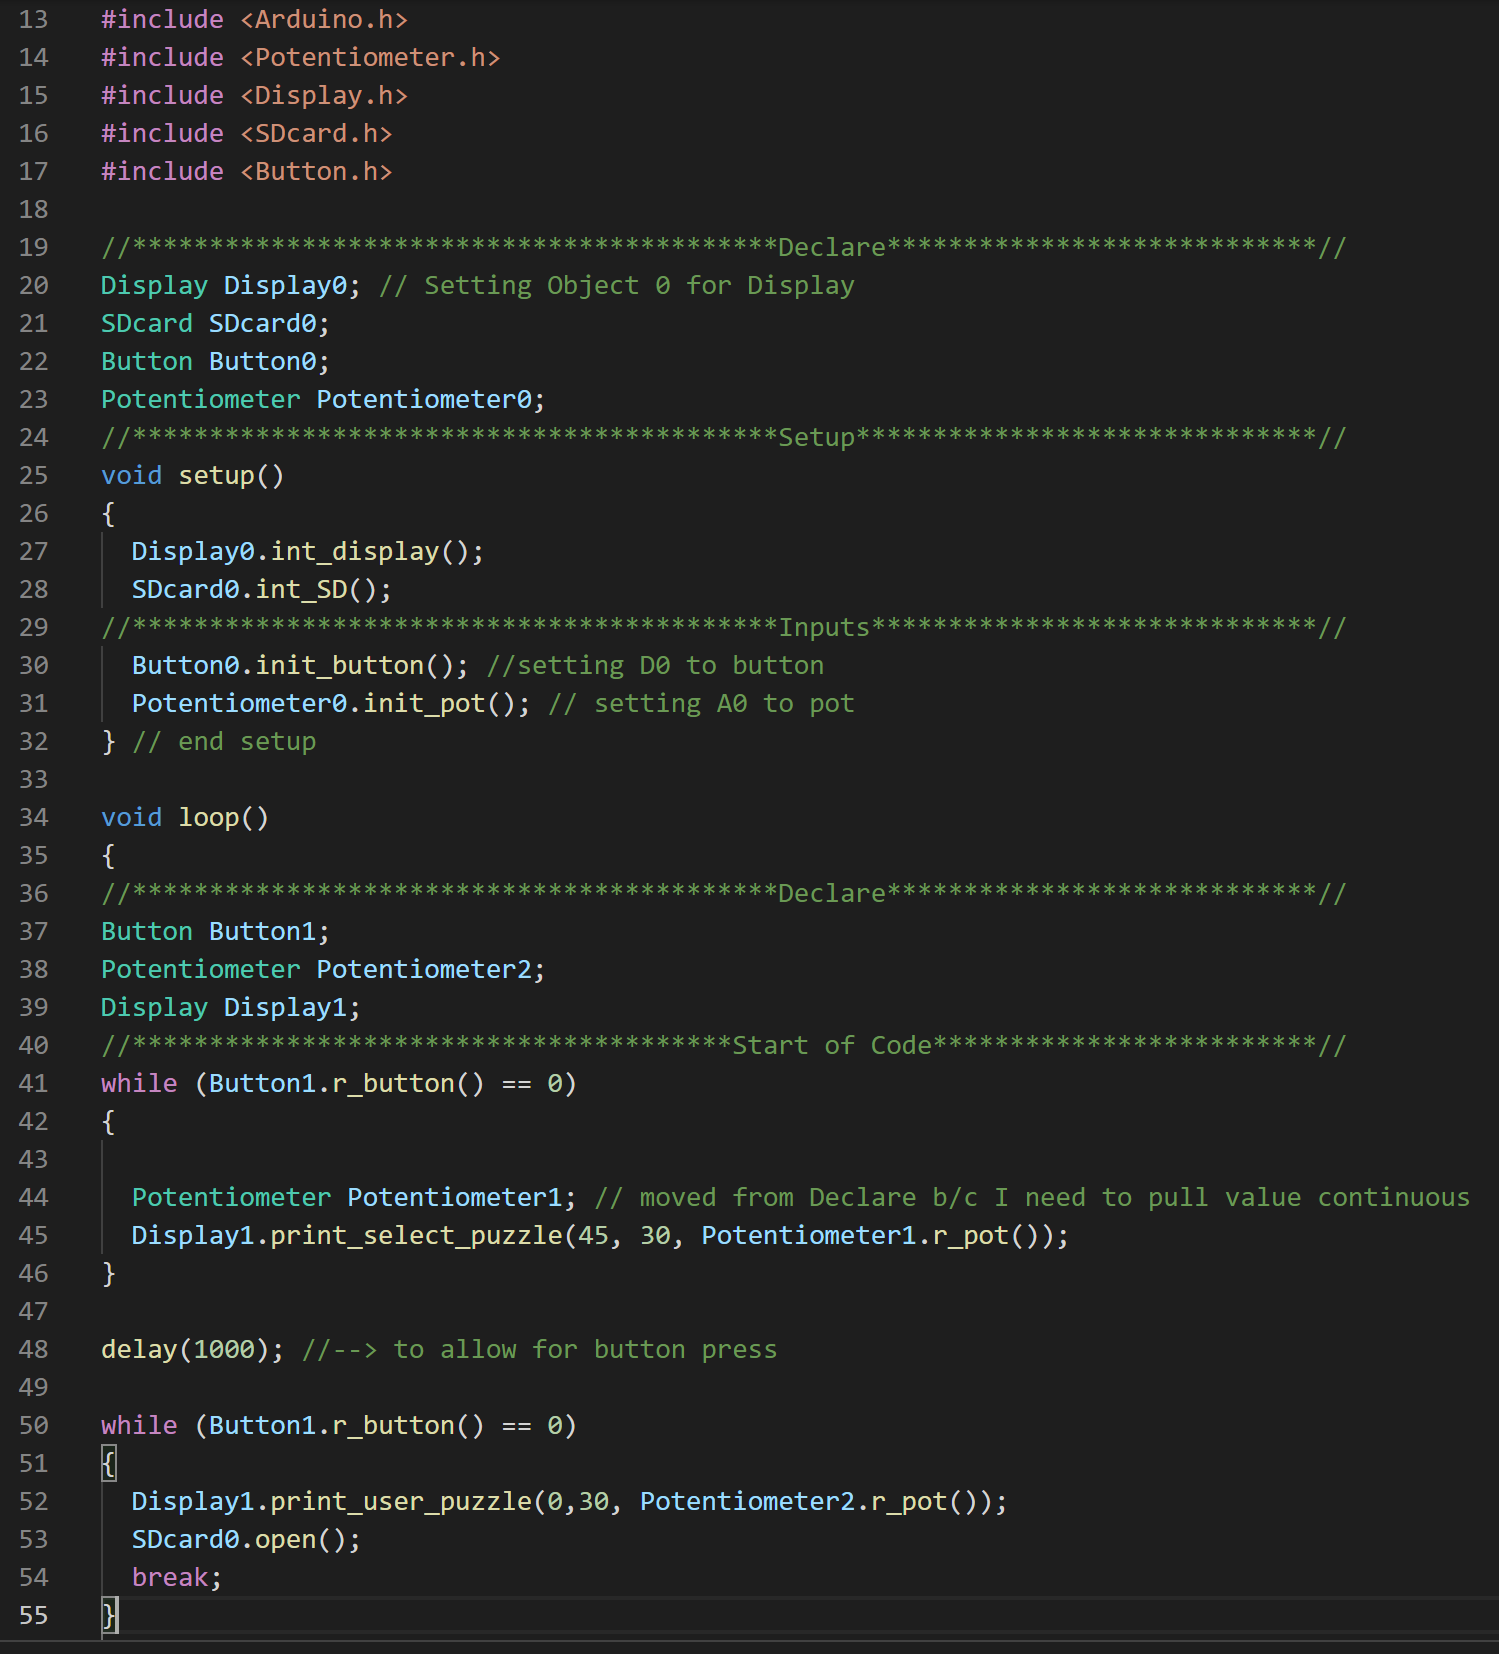
\includegraphics[width=\linewidth]{./Pics/maincpp.PNG}
  \caption{Puzzle me Chess - main.cpp file}
  \label{fig:main}
\end{figure}

\subsection{Display}

\begin{figure}
  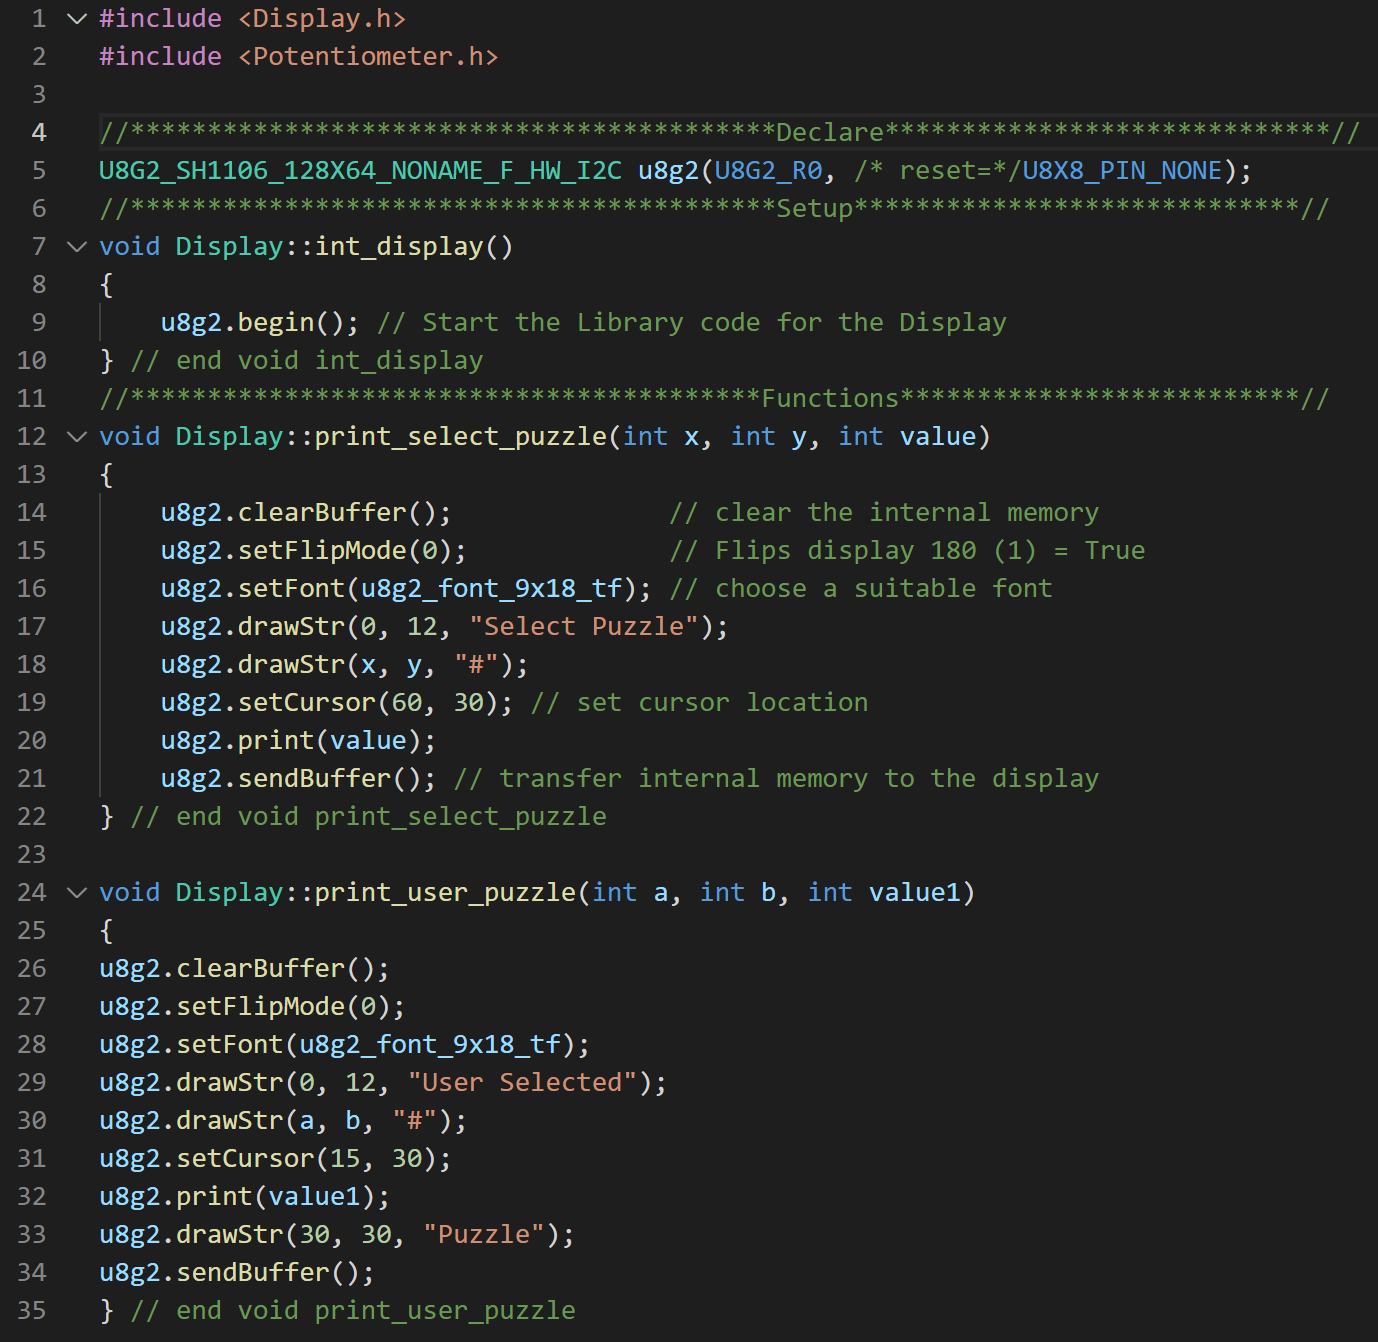
\includegraphics[width=\linewidth]{./Pics/Displaycpp.PNG}
  \caption{Puzzle me Chess - display.cpp file}
  \label{fig:Display}
\end{figure}

\subsection{SDcard}

\begin{figure}
  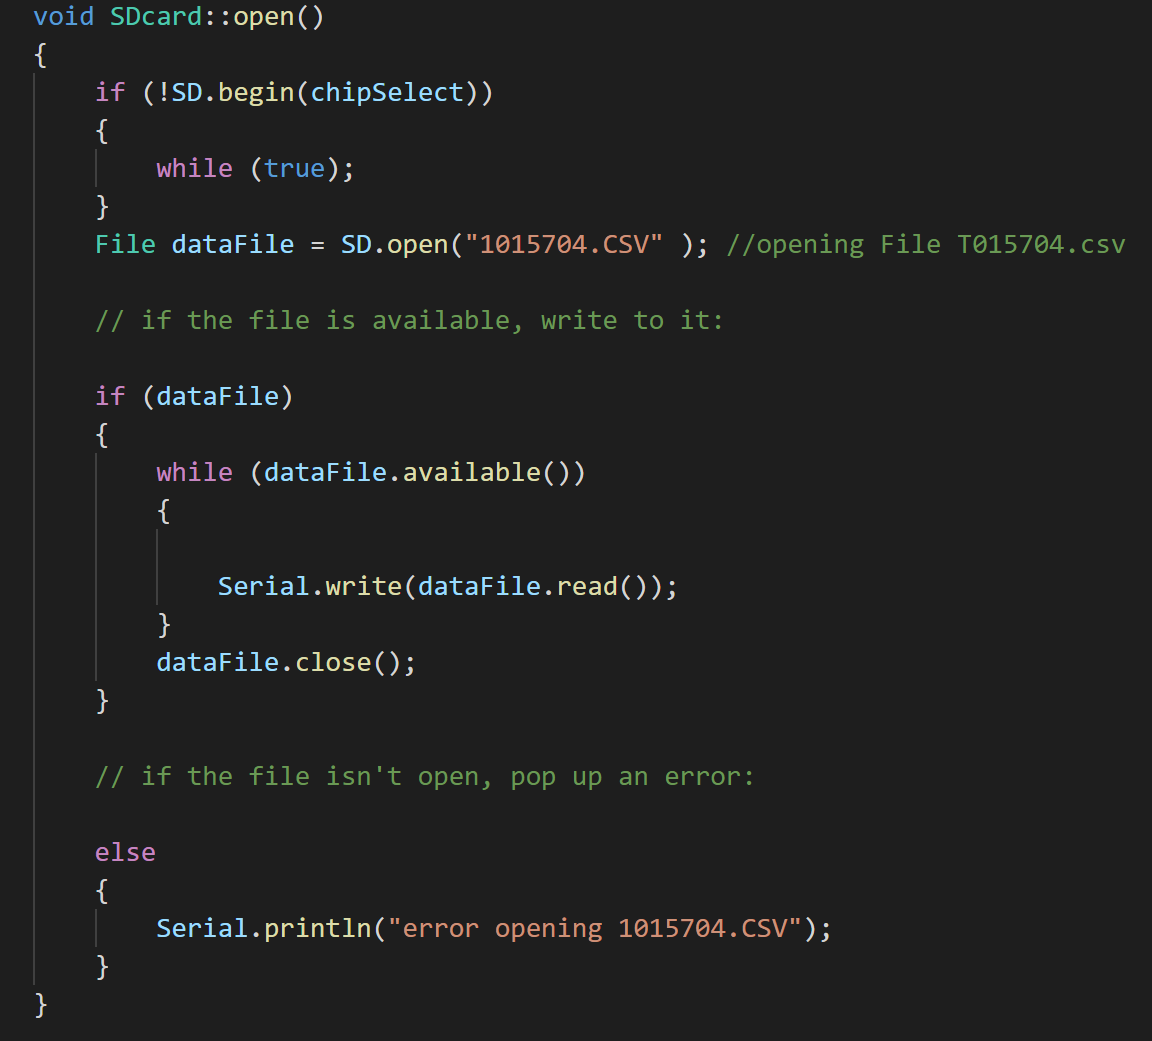
\includegraphics[width=\linewidth]{./Pics/sdcardpart3.PNG}
  \caption{Puzzle me Chess - SDcard.cpp file}
  \label{fig:sdcard1}
\end{figure}

\subsection{Button}

\begin{figure}
  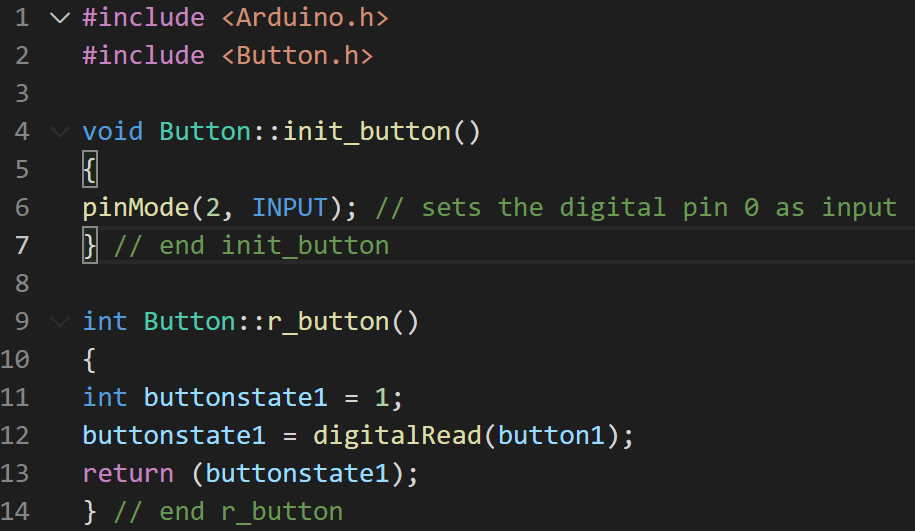
\includegraphics[width=\linewidth]{./Pics/buttoncpp.PNG}
  \caption{Puzzle me Chess - button.cpp file}
  \label{fig:button}
\end{figure}

\subsection{Potentiometer}

\begin{figure}
  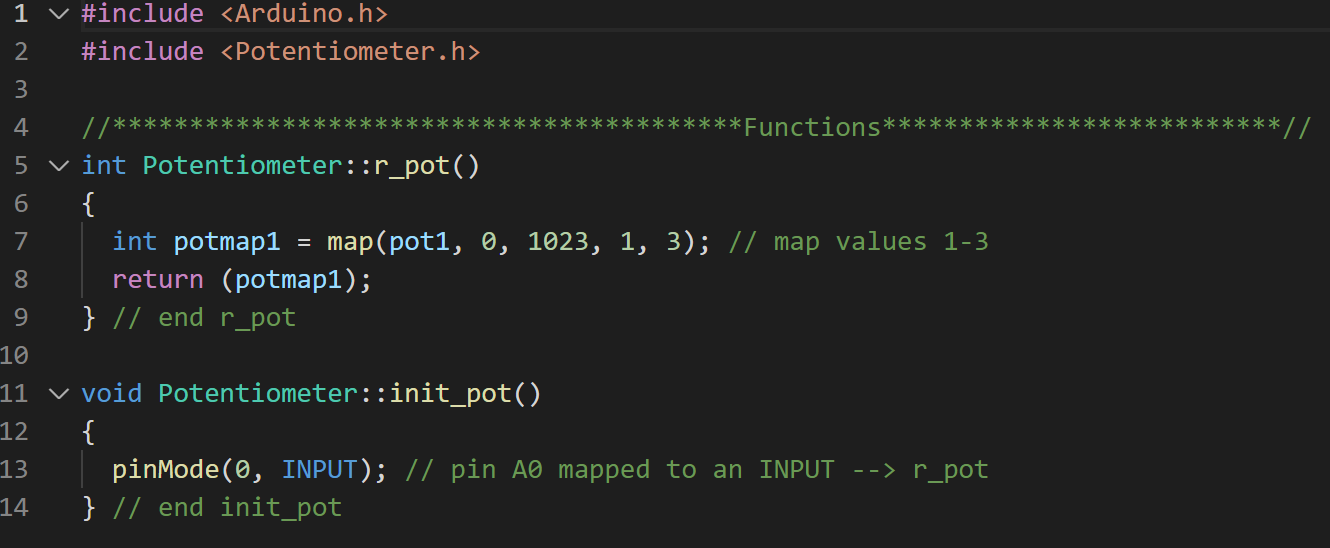
\includegraphics[width=\linewidth]{./Pics/Potentiometercpp.PNG}
  \caption{Puzzle me Chess - Photentiometer.cpp file}
  \label{fig:Photentiometer}
\end{figure}

\section{Material and resource requirements}
\subsection{List of Items (BOM)}
\subsection{Test equipment}
\subsection{Ording from}
include date and times and websites

\section{Development Plan and Schedule}
\subsection{Order of Development}
\subsection{Milestones and Schedule}
\subsection{Risk}

\section{Reference}

\end{document}
